\documentclass[a4paper,12pt]{article}

\input{../../Preambulo.tex}
\newcommand{\assunto}{GEOMETRIA ANALÍTICA}
\newcommand{\atividade}{lista} % prova ou lista
\newcommand{\turma}{INFORMÁTICA 3.\textordmasculine\ ANO}
\newcommand{\numProva}{A}
\newcommand{\professor}{Igor Martins Silva}
\newcommand{\bimestre}{2}
\newcommand{\ano}{2026}
\newcommand{\mesTexto}{junho}
\newcommand{\mesNum}{06}
\newcommand{\dia}{26}
\newcommand{\dataTexto}{\dia\ de \mesTexto\ de \ano}
\newcommand{\dataNun}{\dia/\mesNum/\ano}

\newcommand{\titulo}{}

\ifdefstring{\atividade}{prova}
  {\renewcommand{\titulo}{Avaliação de Matemática}}
{
\ifdefstring{\atividade}{lista}
  {\renewcommand{\titulo}{Lista de exercícios de Matemática}}
{
\ifdefstring{\atividade}{as}
  {\renewcommand{\titulo}{Avaliação Somativa}}
{
\ifdefstring{\atividade}{ad}
  {\renewcommand{\titulo}{Avaliação Diagnóstica}}
  {\renewcommand{\titulo}{Atividade de Matemática}}
}}}

\newcommand{\emtipo}{%
  \ifdefstring{\tipo}{individual}{\tipo}{em \tipo}%
}

\newcommand{\subtitulobase}[3]{%
    % #1 = título da 1ª coluna
    % #2 = conteúdo da 1ª coluna
    % #3 = mostra número da prova? (vazio ou algo)
    
    \begin{center}
        CEFET-MG -- Campus Contagem \\[3pt]
        \titulo\ -- \bimestre.\textordmasculine\ bimestre de \ano \\[3pt]
        \professor
    \end{center}
    
    \begin{center}
        \vspace{15pt}
        \begin{tabular}{|C{210pt}|C{70pt}|C{210pt}|}
            \hline
            \textbf{#1} &
            \textbf{DATA} &
            \textbf{TURMA} \\
            \hline
            #2 & \dataNun & \turma \\
            \hline
        \end{tabular}
    \end{center}
    
    #3
    
    \vspace{15pt}
}

\newcommand{\subtitulolis}{%
  \subtitulobase{ASSUNTO}{\assunto}{}%
}

\newcommand{\subtitulopr}{%
  \subtitulobase{ASSUNTO}{\assunto}{\boxed{\numProva}}%
}

\newcommand{\subtituloas}{%
  \subtitulobase{DISCIPLINA}{MATEMÁTICA}{}%
}

\newcommand{\subtituload}{%
  \subtitulobase{DISCIPLINA}{MATEMÁTICA}{}%
}

\newcommand{\valorquestao}{}

\newenvironment{exercicioBanco}[1][]{%
    \ifdefstring{\atividade}{prova}{%
        \begin{exercicio}[#1]%
    }{%
        \begin{exercicio}%
    }%
}{%
    \end{exercicio}
}

\ifdefstring{\atividade}{lista}{
    \pagecolor{background-color}
}{
    
}



\hypersetup{
    pdfauthor={\professor},
    pdftitle={\titulo \ -- \assunto \ -- \turma},
}

\title{\titulo \ -- \assunto \ -- \turma}
\author{\professor}
\date{\data}

\graphicspath{
    {../../GeometriaAnalitica/}
}

%************* INÍCIO DO DOCUMENTO *************
\begin{document}
    \subtitulolis
        
    \phantomsection
    \addcontentsline{toc}{section}{Exercício 1}
    %%%%%%%%%%%%%%%%%%%%%%%%%%%%%%%%%
%
%       EXERCÍCIO
%
%%%%%%%%%%%%%%%%%%%%%%%%%%%%%%%%%

\ifdefstring{\atividade}{prova}{%
    \ifdefstring{\modo}{objetivo}{%
        \renewcommand{\valorquestao}{\ValorQObj\ ponto}
    }{%
        \renewcommand{\valorquestao}{\ValorQDisc\ pontos}
    }%
}%

\begin{exercicioBanco}[\valorquestao]
Sejam \(A = (-4,-2)\), \(B = (1,3)\) e \(M = (a,b)\) pontos do plano cartesiano. Se \(M\) é o ponto médio de \(\overline{AB}\), determine o valor de \(a+b\).

% Define as alternativas
\newcommand{\alternativas}{%
    \begin{center}
        \begin{tabularx}{\textwidth}{XXXXX}
            (a) \(-2\). &
            (b) \(-1\). &
            (c) \(1\). &
            (d) \(2\). &
            (e) \(3\).
        \end{tabularx}
    \end{center}
}

% Define a resposta correta
\newcommand{\resposta}{B}

% Lógica condicional para exibição
\ifdefstring{\atividade}{lista}{%
    \alternativas
    \vspace{0.5em}
    
    \noindent\textbf{Resposta:} letra \textbf{\resposta}.
}{%
    \ifdefstring{\modo}{objetivo}{%
        \alternativas
    }{%
        % modo = discursiva → não mostra alternativas
    }
}
\end{exercicioBanco}

    \noindent\rule{\linewidth}{1pt}  % linha horizontal fina
    
    \phantomsection
    \addcontentsline{toc}{section}{Exercício 2}
    %%%%%%%%%%%%%%%%%%%%%%%%%%%%%%%%%
%
%       EXERCÍCIO
%
%%%%%%%%%%%%%%%%%%%%%%%%%%%%%%%%%

\ifdefstring{\atividade}{prova}{%
    \ifdefstring{\modo}{objetivo}{%
        \renewcommand{\valorquestao}{\ValorQObj\ ponto}
    }{%
        \renewcommand{\valorquestao}{\ValorQDisc\ pontos}
    }%
}%

\begin{exercicioBanco}[\valorquestao]
Os vértices da base de um triângulo isósceles são os pontos \((1, -1)\) e \((-3, 4)\) de um sistema de coordenadas cartesianas retangulares. Qual a ordenada do terceiro vértice, se ele pertence ao eixo das ordenadas?

% Define as alternativas
\newcommand{\alternativas}{%
    \begin{center}
        \begin{tabularx}{\textwidth}{XXXXX}
            (a) \(\dfrac{23}{10}\). &
            (b) \(\dfrac{13}{9}\). &
            (c) \(\dfrac{15}{7}\). &
            (d) \(\dfrac{21}{11}\). &
            (e) \(\dfrac{19}{2}\).
        \end{tabularx}
    \end{center}
}

% Define a resposta correta
\newcommand{\resposta}{A}

% Lógica condicional para exibição
\ifdefstring{\atividade}{lista}{%
    \alternativas
    \vspace{0.5em}
    
    \noindent\textbf{Resposta:} letra \textbf{\resposta}.
}{%
    \ifdefstring{\modo}{objetivo}{%
        \alternativas
    }{%
        % modo = discursiva → não mostra alternativas
    }
}
\end{exercicioBanco}


    \noindent\rule{\linewidth}{1pt}  % linha horizontal fina
    
    \phantomsection
    \addcontentsline{toc}{section}{Exercício 3}
    \input{../GA_Exercicio3_1}
    \noindent\rule{\linewidth}{1pt}  % linha horizontal fina
    
    \phantomsection
    \addcontentsline{toc}{section}{Exercício 4}
    %%%%%%%%%%%%%%%%%%%%%%%%%%%%%%%%%
%
%       EXERCÍCIO
%
%%%%%%%%%%%%%%%%%%%%%%%%%%%%%%%%%

\ifdefstring{\atividade}{prova}{%
    \ifdefstring{\modo}{objetivo}{%
        \renewcommand{\valorquestao}{\ValorQObj\ ponto}
    }{%
        \renewcommand{\valorquestao}{\ValorQDisc\ pontos}
    }%
}%

\begin{exercicioBanco}[\valorquestao]
Uma das extremidades de um segmento de reta é o ponto \(A = (-2, -2)\). Sabendo que \(M = (3, -2)\) é o ponto médio desse segmento de reta, calcule as coordenadas do ponto \(B = (x, y)\), que é a outra extremidade do segmento de reta.

% Define as alternativas
\newcommand{\alternativas}{%
    \begin{center}
        \begin{tabularx}{\textwidth}{XXXXX}
            (a) \(x = 6\) e \(y = -2\). &
            (b) \(x = 8\) e \(y = 6\). &
            (c) \(x = 8\) e \(y = -2\). &
            (d) \(x = -2\) e \(y = 8\). &
            (e) \(x = 4\) e \(y = 6\).
        \end{tabularx}
    \end{center}
}

% Define a resposta correta
\newcommand{\resposta}{C}

% Lógica condicional para exibição
\ifdefstring{\atividade}{lista}{%
    \alternativas
    \vspace{0.5em}
    
    \noindent\textbf{Resposta:} letra \textbf{\resposta}.
}{%
    \ifdefstring{\modo}{objetivo}{%
        \alternativas
    }{%
        % modo = discursiva → não mostra alternativas
    }
}
\end{exercicioBanco}


    \noindent\rule{\linewidth}{1pt}  % linha horizontal fina
    
    \phantomsection
    \addcontentsline{toc}{section}{Exercício 5}
    %%%%%%%%%%%%%%%%%%%%%%%%%%%%%%%%%
%
%       EXERCÍCIO
%
%%%%%%%%%%%%%%%%%%%%%%%%%%%%%%%%%

\ifdefstring{\atividade}{prova}{%
    \ifdefstring{\modo}{objetivo}{%
        \renewcommand{\valorquestao}{\ValorQObj\ ponto}
    }{%
        \renewcommand{\valorquestao}{\ValorQDisc\ pontos}
    }%
}%

\begin{exercicioBanco}[\valorquestao]
Para cada afirmativa abaixo, assinale se ela é verdadeira (V) ou falsa (F).
%
\begin{enumerate}[\(\bullet\)]
    \item \(A = (0,2)\), \(B = (-3,1)\) e \(C = (4,5)\) estão alinhados.
    %
    \item \(P = (2,3)\) pertence à reta que contém os pontos \(A = (1,1)\) e \(B = (0,-3)\).
    %
    \item As retas \(r\) e \(s\) determinadas, respectivamente, pelas equações \(15x + 10y - 3 = 0\) e \(9x + 6y - 1 = 0\) são paralelas.
    %
    \item A distância entre o ponto \(P = (0,3)\) e a reta \(r: 4x + 3y + 1 = 0\) é \(2\).
\end{enumerate}
%

% Define as alternativas
\newcommand{\alternativas}{%
    \begin{center}
        \begin{tabularx}{\textwidth}{XXXXX}
            (a) (V, F, F, V). &
            (b) (V, F, F, F). &
            (c) (F, V, V, F). &
            (d) (F, F, V, V). &
            (e) (F, V, F, V).
        \end{tabularx}
    \end{center}
}

% Define a resposta correta
\newcommand{\resposta}{D}

% Lógica condicional para exibição
\ifdefstring{\atividade}{lista}{%
    \alternativas
    \vspace{0.5em}
    
    \noindent\textbf{Resposta:} letra \textbf{\resposta}.
}{%
    \ifdefstring{\modo}{objetivo}{%
        \alternativas
    }{%
        % modo = discursiva → não mostra alternativas
    }
}
\end{exercicioBanco}


    \noindent\rule{\linewidth}{1pt}  % linha horizontal fina
    
    \phantomsection
    \addcontentsline{toc}{section}{Exercício 6}
    %%%%%%%%%%%%%%%%%%%%%%%%%%%%%%%%%
%
%       EXERCÍCIO
%
%%%%%%%%%%%%%%%%%%%%%%%%%%%%%%%%%

\ifdefstring{\atividade}{prova}{%
    \ifdefstring{\modo}{objetivo}{%
        \renewcommand{\valorquestao}{\ValorQObj\ ponto}
    }{%
        \renewcommand{\valorquestao}{\ValorQDisc\ pontos}
    }%
}%

\begin{exercicioBanco}[\valorquestao]
A figura a seguir ilustra as representações cartesianas das retas $r$ e $s$ de equações $y = x + 3$ e $y = -3x + 27$, respectivamente, com $x$ e $y$ dados em metros. Determine a área, em metros quadrados, do quadrilátero destacado.

\begin{center}
    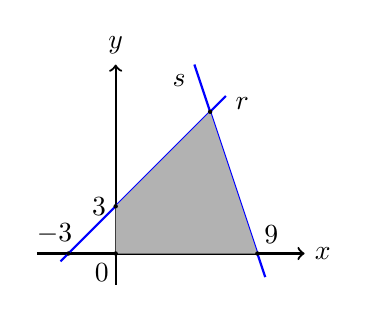
\begin{tikzpicture}[scale=0.2]
        % Eixos
        \draw[->,thick] (-5,0) -- (12,0) node[right] {$x$};
        \draw[->,thick] (0,-2) -- (0,12) node[above] {$y$};

        % Retas
        \draw[domain=-3.5:7, smooth, variable=\x, blue, thick] 
        plot ({\x}, {\x+3});
        
        \draw[domain=5:9.5, smooth, variable=\x, blue, thick] 
        plot ({\x}, {-3*\x+27});

        % Quadrilátero sombreado
        \fill[gray!60]
        (0,0) --
        (0,3) --
        (6,9) --
        (9,0) -- cycle;

        % Marcas no eixo x
        \node[left, above, xshift=-5pt] at (-3,0) {$-3$};
        \node[left, below, xshift=-5pt] at (0,0) {$0$};
        \node[right, above, xshift=5pt] at (9,0) {$9$};

        % Marca no eixo y
        \node[left] at (0,3) {$3$};

        % Identificação das retas
        \node[right] at (7,9.5) {$r$};
        \node[right] at (3,11) {$s$};
        
        % Pontos importantes
        \fill (0,0) circle (4pt);
        \fill (0,3) circle (4pt);
        \fill (6,9) circle (4pt);
        \fill (9,0) circle (4pt);
        \fill (-3,0) circle (4pt);
    \end{tikzpicture}
\end{center}



% Define as alternativas
\newcommand{\alternativas}{%
    \begin{center}
        \begin{tabularx}{\textwidth}{XXXXX}
            (a) \(49,5\) m\(^{2}\). &
            (b) \(49\) m\(^{2}\). &
            (c) \(48,5\) m\(^{2}\). &
            (d) \(48\) m\(^{2}\). &
            (e) \(47,5\) m\(^{2}\).
        \end{tabularx}
    \end{center}
}

% Define a resposta correta
\newcommand{\resposta}{A}

% Lógica condicional para exibição
\ifdefstring{\atividade}{lista}{%
    \alternativas
    \vspace{0.5em}
    
    \noindent\textbf{Resposta:} letra \textbf{\resposta}.
}{%
    \ifdefstring{\modo}{objetivo}{%
        \alternativas
    }{%
        % modo = discursiva → não mostra alternativas
    }
}
\end{exercicioBanco}


    \noindent\rule{\linewidth}{1pt}  % linha horizontal fina
    
    \phantomsection
    \addcontentsline{toc}{section}{Exercício 7}
    %%%%%%%%%%%%%%%%%%%%%%%%%%%%%%%%%
%
%       EXERCÍCIO
%
%%%%%%%%%%%%%%%%%%%%%%%%%%%%%%%%%

\ifdefstring{\atividade}{prova}{%
    \ifdefstring{\modo}{objetivo}{%
        \renewcommand{\valorquestao}{\ValorQObj\ ponto}
    }{%
        \renewcommand{\valorquestao}{\ValorQDisc\ pontos}
    }%
}%

\begin{exercicioBanco}[\valorquestao]
Determine \(m\) para que as retas \(m^{2}x + my + 8 = 0\) e \(3x + (m+1)y + 9 = 0\) sejam perpendiculares.

% Define as alternativas
\newcommand{\alternativas}{%
    \begin{center}
        \begin{tabularx}{\textwidth}{XXXXX}
            (a) \(\dfrac{1}{2}\). &
            (b) \(\dfrac{2}{3}\). &
            (c) \(-\dfrac{1}{4}\). &
            (d) \(\dfrac{3}{4}\). &
            (e) \(\dfrac{2}{5}\).
        \end{tabularx}
    \end{center}
}

% Define a resposta correta
\newcommand{\resposta}{C}

% Lógica condicional para exibição
\ifdefstring{\atividade}{lista}{%
    \alternativas
    \vspace{0.5em}
    
    \noindent\textbf{Resposta:} letra \textbf{\resposta}.
}{%
    \ifdefstring{\modo}{objetivo}{%
        \alternativas
    }{%
        % modo = discursiva → não mostra alternativas
    }
}
\end{exercicioBanco}


    \noindent\rule{\linewidth}{1pt}  % linha horizontal fina
    
    \phantomsection
    \addcontentsline{toc}{section}{Exercício 8}
    %%%%%%%%%%%%%%%%%%%%%%%%%%%%%%%%%
%
%       EXERCÍCIO
%
%%%%%%%%%%%%%%%%%%%%%%%%%%%%%%%%%

\ifdefstring{\atividade}{prova}{%
    \ifdefstring{\modo}{objetivo}{%
        \renewcommand{\valorquestao}{\ValorQObj\ ponto}
    }{%
        \renewcommand{\valorquestao}{\ValorQDisc\ pontos}
    }%
}%

\begin{exercicioBanco}[\valorquestao]
Determine o valor numérico de \(k\) para que a distância de um ponto de coordenadas \((2, k)\), situado no primeiro quadrante, à reta de equação \(3x + 4y - 24 = 0\), seja igual a 18 unidades.

% Define as alternativas
\newcommand{\alternativas}{%
    \begin{center}
        \begin{tabularx}{\textwidth}{XXXXX}
            (a) \(18\). &
            (b) \(27\). &
            (c) \(13\). &
            (d) \(33\). &
            (e) \(19\).
        \end{tabularx}
    \end{center}
}

% Define a resposta correta
\newcommand{\resposta}{B}

% Lógica condicional para exibição
\ifdefstring{\atividade}{lista}{%
    \alternativas
    \vspace{0.5em}
    
    \noindent\textbf{Resposta:} letra \textbf{\resposta}.
}{%
    \ifdefstring{\modo}{objetivo}{%
        \alternativas
    }{%
        % modo = discursiva → não mostra alternativas
    }
}
\end{exercicioBanco}


    \noindent\rule{\linewidth}{1pt}  % linha horizontal fina
    
    \phantomsection
    \addcontentsline{toc}{section}{Exercício 9}
    %%%%%%%%%%%%%%%%%%%%%%%%%%%%%%%%%
%
%       EXERCÍCIO
%
%%%%%%%%%%%%%%%%%%%%%%%%%%%%%%%%%

\ifdefstring{\atividade}{prova}{%
    \ifdefstring{\modo}{objetivo}{%
        \renewcommand{\valorquestao}{\ValorQObj\ ponto}
    }{%
        \renewcommand{\valorquestao}{\ValorQDisc\ pontos}
    }%
}%

\begin{exercicioBanco}[\valorquestao]
Duas retas \(r\) e \(s\) são dadas, respectivamente, pelas equações \(3x - 4y = 3\) e \(2x + y = 2\). Um ponto \(P\) pertencente à reta \(s\) tem abcissa positiva e dista 22 unidades de medida da reta \(r\). Se \(ax + by + c = 0\) é a equação da reta que contém \(P\) e é paralela a \(r\), então, qual o valor de \(a + b + c\)?

% Define as alternativas
\newcommand{\alternativas}{%
    \begin{center}
        \begin{tabularx}{\textwidth}{XXXXX}
            (a) \(57\). &
            (b) \(-96\). &
            (c) \(142\). &
            (d) \(-19\). &
            (e) \(-114\).
        \end{tabularx}
    \end{center}
}

% Define a resposta correta
\newcommand{\resposta}{E}

% Lógica condicional para exibição
\ifdefstring{\atividade}{lista}{%
    \alternativas
    \vspace{0.5em}
    
    \noindent\textbf{Resposta:} letra \textbf{\resposta}.
}{%
    \ifdefstring{\modo}{objetivo}{%
        \alternativas
    }{%
        % modo = discursiva → não mostra alternativas
    }
}
\end{exercicioBanco}


    \noindent\rule{\linewidth}{1pt}  % linha horizontal fina
    
    \phantomsection
    \addcontentsline{toc}{section}{Exercício 10}
    %%%%%%%%%%%%%%%%%%%%%%%%%%%%%%%%%
%
%       EXERCÍCIO
%
%%%%%%%%%%%%%%%%%%%%%%%%%%%%%%%%%

\ifdefstring{\atividade}{prova}{%
    \ifdefstring{\modo}{objetivo}{%
        \renewcommand{\valorquestao}{\ValorQObj\ ponto}
    }{%
        \renewcommand{\valorquestao}{\ValorQDisc\ pontos}
    }%
}%

\begin{exercicioBanco}[\valorquestao]
Sejam \(A\) e \(B\) dois pontos da reta de equação \(y = 2x + 2\), que distam duas unidades da origem. Neste caso, qual a soma das abscissas de \(A\) e \(B\)?

% Define as alternativas
\newcommand{\alternativas}{%
    \begin{center}
        \begin{tabularx}{\textwidth}{XXXXX}
            (a) \(-\dfrac{1}{3}\). &
            (b) \(\dfrac{5}{8}\). &
            (c) \(\dfrac{5}{2}\). &
            (d) \(-\dfrac{8}{5}\). &
            (e) \(-\dfrac{8}{3}\).
        \end{tabularx}
    \end{center}
}

% Define a resposta correta
\newcommand{\resposta}{D}

% Lógica condicional para exibição
\ifdefstring{\atividade}{lista}{%
    \alternativas
    \vspace{0.5em}
    
    \noindent\textbf{Resposta:} letra \textbf{\resposta}.
}{%
    \ifdefstring{\modo}{objetivo}{%
        \alternativas
    }{%
        % modo = discursiva → não mostra alternativas
    }
}
\end{exercicioBanco}


    \noindent\rule{\linewidth}{1pt}  % linha horizontal fina
    
    \phantomsection
    \addcontentsline{toc}{section}{Exercício 11}
    %%%%%%%%%%%%%%%%%%%%%%%%%%%%%%%%%
%
%       EXERCÍCIO
%
%%%%%%%%%%%%%%%%%%%%%%%%%%%%%%%%%

\ifdefstring{\atividade}{prova}{%
    \ifdefstring{\modo}{objetivo}{%
        \renewcommand{\valorquestao}{\ValorQObj\ ponto}
    }{%
        \renewcommand{\valorquestao}{\ValorQDisc\ pontos}
    }%
}%

\begin{exercicioBanco}[\valorquestao]
A circunferência de equação \(x^{2} + y^{2} - 4x - 2y - 4 = 0\) intersecta o eixo das abscissas nos pontos \(M\) e \(N\). Qual a distância entre \(M\) e \(N\)?

% Define as alternativas
\newcommand{\alternativas}{%
    \begin{center}
        \begin{tabularx}{\textwidth}{XXXXX}
            (a) \(4\sqrt{2}\). &
            (b) \(2\sqrt{5}\). &
            (c) \(\sqrt{2}\). &
            (d) \(4\sqrt{3}\). &
            (e) \(3\sqrt{2}\).
        \end{tabularx}
    \end{center}
}

% Define a resposta correta
\newcommand{\resposta}{A}

% Lógica condicional para exibição
\ifdefstring{\atividade}{lista}{%
    \alternativas
    \vspace{0.5em}
    
    \noindent\textbf{Resposta:} letra \textbf{\resposta}.
}{%
    \ifdefstring{\modo}{objetivo}{%
        \alternativas
    }{%
        % modo = discursiva → não mostra alternativas
    }
}
\end{exercicioBanco}


    \noindent\rule{\linewidth}{1pt}  % linha horizontal fina
    
    \phantomsection
    \addcontentsline{toc}{section}{Exercício 12}
    %%%%%%%%%%%%%%%%%%%%%%%%%%%%%%%%%
%
%       EXERCÍCIO
%
%%%%%%%%%%%%%%%%%%%%%%%%%%%%%%%%%

\ifdefstring{\atividade}{prova}{%
    \ifdefstring{\modo}{objetivo}{%
        \renewcommand{\valorquestao}{\ValorQObj\ ponto}
    }{%
        \renewcommand{\valorquestao}{\ValorQDisc\ pontos}
    }%
}%

\begin{exercicioBanco}[\valorquestao]
Determine a equação da circunferência de centro \(C = (5,-5)\) e que contém o ponto \(P = (0,-5)\).

% Define as alternativas
\newcommand{\alternativas}{%
    \begin{center}
        \begin{tabularx}{\textwidth}{XXX}
            (a) \(\dfrac{x^{2}}{5} + \dfrac{y^{2}}{5} - 2x + 2y + 5 = 0\). &
            (b) \(x^{2} - 10x + y^{2} + 10y = 25\). &
            (c) \(x^{2} - x + y^{2} - y - 5 = 0\). \\[15pt]
            (d) \(5x^{2} + 5y^{2} - x - y = 25\). &
            (e) \(5x^{2} + 5y^{2} + x + y = 25\).
        \end{tabularx}
    \end{center}
}

% Define a resposta correta
\newcommand{\resposta}{A}

% Lógica condicional para exibição
\ifdefstring{\atividade}{lista}{%
    \alternativas
    \vspace{0.5em}
    
    \noindent\textbf{Resposta:} letra \textbf{\resposta}.
}{%
    \ifdefstring{\modo}{objetivo}{%
        \alternativas
    }{%
        % modo = discursiva → não mostra alternativas
    }
}
\end{exercicioBanco}


    \noindent\rule{\linewidth}{1pt}  % linha horizontal fina
    
    \phantomsection
    \addcontentsline{toc}{section}{Exercício 13}
    %%%%%%%%%%%%%%%%%%%%%%%%%%%%%%%%%
%
%       EXERCÍCIO
%
%%%%%%%%%%%%%%%%%%%%%%%%%%%%%%%%%

\ifdefstring{\atividade}{prova}{%
    \ifdefstring{\modo}{objetivo}{%
        \renewcommand{\valorquestao}{\ValorQObj\ ponto}
    }{%
        \renewcommand{\valorquestao}{\ValorQDisc\ pontos}
    }%
}%

\begin{exercicioBanco}[\valorquestao]
Em relação às circunferência \(C_{1}: x^{2} + y^{2} - 2x - 2y - 8 = 0\) e \(C_{2}: x^{2} + y^{2} + 10x + 2y + 16 = 0\), é correto afirmar que são:

% Define as alternativas
\newcommand{\alternativas}{%
    \begin{center}
        \begin{tabularx}{\textwidth}{XXX}
            (a) exteriores. &
            (b) tangentes exteriormente. &
            (c) secantes. \\[5pt]
            (d) tangentes interiormente. &
            (e) interiores.
        \end{tabularx}
    \end{center}
}

% Define a resposta correta
\newcommand{\resposta}{B}

% Lógica condicional para exibição
\ifdefstring{\atividade}{lista}{%
    \alternativas
    \vspace{0.5em}
    
    \noindent\textbf{Resposta:} letra \textbf{\resposta}.
}{%
    \ifdefstring{\modo}{objetivo}{%
        \alternativas
    }{%
        % modo = discursiva → não mostra alternativas
    }
}
\end{exercicioBanco}


    \noindent\rule{\linewidth}{1pt}  % linha horizontal fina
    
    \phantomsection
    \addcontentsline{toc}{section}{Exercício 14}
    %%%%%%%%%%%%%%%%%%%%%%%%%%%%%%%%%
%
%       EXERCÍCIO
%
%%%%%%%%%%%%%%%%%%%%%%%%%%%%%%%%%

\ifdefstring{\atividade}{prova}{%
    \ifdefstring{\modo}{objetivo}{%
        \renewcommand{\valorquestao}{\ValorQObj\ ponto}
    }{%
        \renewcommand{\valorquestao}{\ValorQDisc\ pontos}
    }%
}%

\begin{exercicioBanco}[\valorquestao]
Na figura estão representadas, em um plano cartesiano, duas circunferências: \(C_{1}\) (de raio 3 e centro \(O_{1}\)) e  \(C_{2}\) (de raio 1 e centro \(O_{2}\)), tangentes entre si, e uma reta \(t\) tangente às duas circunferências nos pontos \(P\) e \(Q\).

\begin{center}
    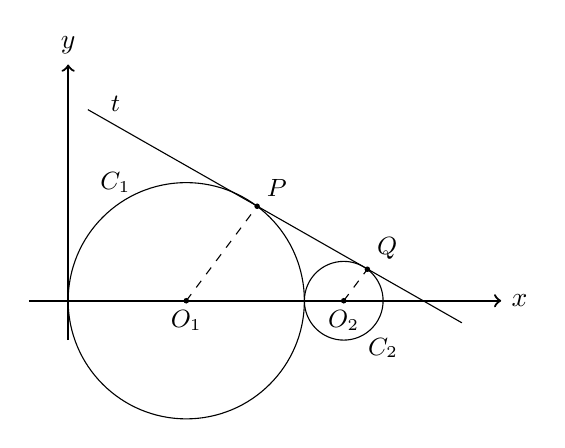
\begin{tikzpicture}[scale=0.5]
        % Eixos
        \draw[->,thick] (-1,0) -- (11,0) node[right] {$x$};
        \draw[->,thick] (0,-1) -- (0,6) node[above] {$y$};

        % Centros
        \coordinate (O1) at (3,0);
        \coordinate (O2) at (7,0);

        % Raios
        \def\rA{3}
        \def\rB{1}

        % Círculos
        \draw (O1) circle (\rA);
        \draw (O2) circle (\rB);

        % Pontos dos centros
        \fill (O1) circle (2pt) node[below] {\small$O_1$};
        \fill (O2) circle (2pt) node[below] {\small$O_2$};

        % Pontos de tangência (aproximados manualmente)
        \draw[domain=0.5:10, smooth, variable=\x]
            plot ({\x}, {-0.57*\x + 5.14});
        
        \node at (1.2,5) {\small$t$};
        
        \coordinate (P) at (4.8,2.4);
        \coordinate (Q) at (7.6,0.8);

        \fill (P) circle (2pt) node[above right] {\small$P$};
        \fill (Q) circle (2pt) node[above right] {\small$Q$};

        % Segmentos pontilhados (raios até a tangente)
        \draw[dashed] (O1) -- (P);
        \draw[dashed] (O2) -- (Q);

        % Rótulos dos círculos
        \node at (1.2,3) {\small$C_1$};
        \node at (8,-1.2) {\small$C_2$};
    \end{tikzpicture}
\end{center}

Nessas condições, determine a equação da reta t.

% Define as alternativas
\newcommand{\alternativas}{%
    \begin{center}
        \begin{tabularx}{\textwidth}{XXX}
            (a) \(y = -\sqrt{3}x + 3\sqrt{3}\). &
            (b) \(y = -\dfrac{\sqrt{3}}{3}x + 3\sqrt{3}\). &
            (c) \(y = -x + 4\). \\[15pt]
            (d) \(y = -\dfrac{2}{3}x + 4\). &
            (e) \(y = -\dfrac{4}{5}x + 4\).
        \end{tabularx}
    \end{center}
}

% Define a resposta correta
\newcommand{\resposta}{B}

% Lógica condicional para exibição
\ifdefstring{\atividade}{lista}{%
    \alternativas
    \vspace{0.5em}
    
    \noindent\textbf{Resposta:} letra \textbf{\resposta}.
}{%
    \ifdefstring{\modo}{objetivo}{%
        \alternativas
    }{%
        % modo = discursiva → não mostra alternativas
    }
}
\end{exercicioBanco}


    \noindent\rule{\linewidth}{1pt}  % linha horizontal fina
\end{document}
%*************** FINAL DO DOCUMENTO ***************
